\documentclass[tikz,border=4pt]{standalone}
\usepackage{fontspec}\usepackage{xcolor}\usetikzlibrary{arrows.meta,calc,positioning}
\setsansfont{Lato}
\begin{document}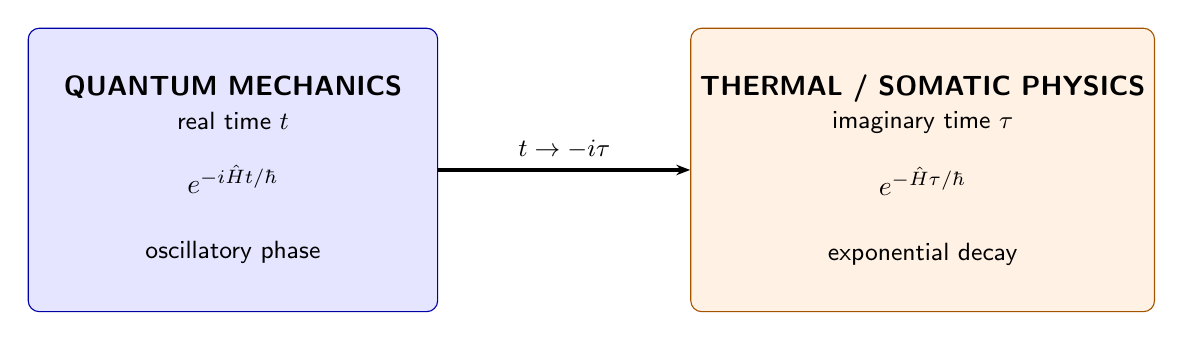
\begin{tikzpicture}[font=\sffamily,box/.style={rounded corners=4pt,draw=#1!65!black,fill=#1!10,minimum width=5.2cm,minimum height=3.6cm,align=center}]
\node[box=blue] (quantum) {\textbf{QUANTUM MECHANICS}\\\small real time $t$\\[4mm]$e^{-i\hat Ht/\hbar}$\\[4mm]\small oscillatory phase};
\node[box=orange,right=3.2cm of quantum] (thermal) {\textbf{THERMAL / SOMATIC PHYSICS}\\\small imaginary time $\tau$\\[4mm]$e^{-\hat H\tau/\hbar}$\\[4mm]\small exponential decay};
\draw[-{Stealth[length=5pt]},line width=1.2pt] (quantum) -- (thermal) node[midway,above,font=\small] {$t\to-i\tau$};
\end{tikzpicture}\end{document}
